\documentclass[a4paper,11pt]{jsarticle} % ceostyを用いるための文書クラス

% 冊子形式にするには表紙(ページ数に含まれない)で
% 1ページ使っているので最後のページのページ番号が
% 4n  ->透かしがしにくい(表紙と裏表紙の裏面が白紙)
% 4n+1->一番微妙
% 4n+2->表紙と白紙の裏表紙ができる---こうなるように調整
% 4n+3->裏表紙も使う

\usepackage{fancyhdr}	% ページスタイル

%%スタイル
% 数式やテキストの描画
\usepackage{amsmath, amsfonts, amssymb, mathtools, mathrsfs, latexsym}	% ams関連は数式書くのに必須!!
%\DeclarePairedDelimiter{\abs}{\lvert}{\rvert}
\usepackage{nccmath, empheq}	% 結構ピンポイントなパッケージ

% 画像
%% 枠だけ表示(Cannot determine size of graphicと結構怒られる)
%\usepackage[draft]{graphicx}
%% 普通に表示させる(ただ重くなりやすい)
\usepackage[dvipdfmx]{graphicx}
\usepackage[dvipdfmx]{color}
\usepackage{here}	% 絶対Hereって勝手に呼んでるやつ
\usepackage{wrapfig}	% 回り込み(ceostyのymawarikomiもある)
\usepackage{subcaption}	% minipageを使って図を並べるときの各画像のキャプションに必要

% このファイルの肝.
% usepackageの順番(ceoとの前後関係)を変えると途端にエラーを吐くので注意
%\usepackage{ceo}
% 以下のパッケージはceostyの煽りをくらったもの
\usepackage{enumerate, comment}	% 順に文書モードでの段落環境, 複数行コメント

\pagestyle{fancy}
  \lhead{2023年10月21日}
  \rhead{第2問}
  \cfoot{}

\newcommand{\vevenspace}{\vspace{\stretch{1}}}	
\newcommand{\hruleline}{\par\noindent\hrulefill\par}
\newcommand{\length}[1]{$\overline{\textup{#1}}$}
\renewcommand{\eq}{$=$}
\newcommand{\vreidai}{\vspace{\stretch{0.3}}}
\newcommand{\nn}{$n$}
\newcommand{\m}{$m$}
\newcommand{\kmath}{$k$}
\renewcommand{\O}{\textup{O}}
\newcommand{\Pn}[2]{$\textup{#1}_{#2}$}
\newcommand{\mathPn}[2]{\textup{#1}_{#2}}
\renewcommand{\P}{\textup{P}}
\newcommand{\Q}{\textup{Q}}
\newcommand{\R}{\textup{R}}
\newcommand{\A}{\textup{A}}
\newcommand{\B}{\textup{B}}
\newcommand{\C}{\textup{C}}
\newcommand{\D}{\textup{D}}
\newcommand{\numseq}[2]{$\{#1_{#2}\}$}
\newcommand{\combi}[2]{{}_{#1}\mathrm{C}_{#2}}
\newcommand{\xy}{$xy$}
\newcommand{\yz}{$yz$}
\newcommand{\xz}{$xz$}
\newcommand{\zx}{$zx$}
\newcommand{\xyz}{$xyz$}
\newcommand{\x}{$x$}
\newcommand{\y}{$y$}
\newcommand{\z}{$z$}
\newcommand{\g}{$g$}


\newcounter{partNo}
\newcommand{\qPart}{
  \pagebreak
  \stepcounter{partNo}
  \noindent \textup{\Large 第\arabic{partNo}問} 
  \par \vspace{0.5\baselineskip}
}

\newcommand{\calcPage}{
  \pagebreak
  \begin{center}
    \textless\,計算用紙\,\textgreater
  \end{center}
  \pagebreak
}

\newcommand{\brankPage}{
  \pagebreak \mbox{} \pagebreak
}

%%%%%%%%%% メイン %%%%%%%%%%%
\begin{document}
%!TEX root = *.tex
%%%%%%%%%%%%%%%%%%
% カウンタのリセット
% 問題文
{
\begin{wrapfigure}{r}{14zw}
  \vspace*{-\intextsep}
  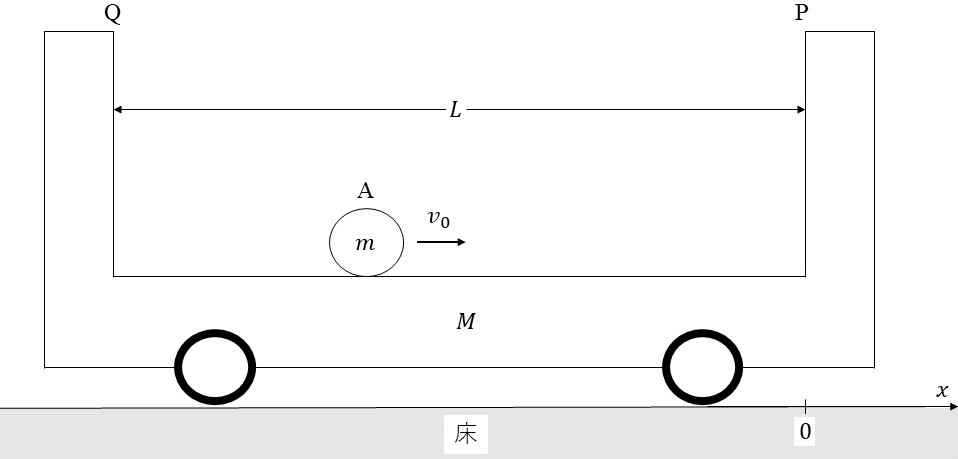
\includegraphics[width=14zw]{../graphs/jumon_42.jpg}
\end{wrapfigure}

図1のように水平な床の上に質量$M$,長さ$L$の台車が静止している.
台車の上には大きさが無視できる質量$m$の小球Aが乗っており,速度$v_0\,(v_0>0)$で運動している.
この問いで使用する速度はすべて床に対する速度であり,麦向きを正とする.
また,摩擦や空気抵抗は無視できるものとする.
\par}

\begin{enumerate}[(1)]
  \setlength{\leftskip}{-1.5zw}
  \setlength{\itemindent}{1zw}\setlength{\labelsep}{0.5zw}
  \setlength{\labelwidth}{1zw}\setlength{\leftmargin}{1zw}
  \setlength{\itemsep}{0.5\baselineskip}
  \item 小球Aが台車両端の壁P,Qに弾性衝突する場合,次の問いに答えよ.
  \begin{enumerate}[(a)]
    \setlength{\leftskip}{-2.5zw}
    \setlength{\itemindent}{1zw}\setlength{\labelsep}{1zw}
    \setlength{\labelwidth}{1zw}
    \item 小球Aが壁Pで最初に台車と衝突した直後の小球および台車の速度(それぞれ$v_1$および$V_1$)を求めよ.
    \item 小球Aは,壁Pで最初に台車と衝突してから時間$T$が経過した後に,壁Qで再び台車と衝突した.このときの時間$T$を求めよ.さらに,壁Qに衝突した直後の小球および台車の速度(それぞれ$v_2$および$V_2$)を求めよ.
    \item $M=m$の場合,小球Aと壁Pの位置の時間変化を$x\mathchar`-t$グラフに実線と点線で示せ.
    ただし,位置は床に固定された座標\x で表し,小球Aが壁Pに最初に衝突した時刻を$t=0$,位置を$x=0$として,$0\leqq t\leqq 3T$の範囲で示せ.
    \item $M=2m$の場合,台車が3Lの距離を進むのに要する時間を求めよ.
  \end{enumerate}
  \item 小球Aが台車両端の壁P,Qに反発係数$e\,(0<e<1)$で非弾性衝突する場合,次の問いに答えよ.
  \begin{enumerate}[(a)]
    \setlength{\leftskip}{-2.5zw}
    \setlength{\itemindent}{1zw}\setlength{\labelsep}{1zw}
    \setlength{\labelwidth}{1zw}
    \item 小球Aが壁Pで最初に台車と衝突した直後の小球および台車の速度(それぞれ${v_1}^\prime$および${V_1}^\prime$)を求めよ.
    \item その後,小球Aは壁Q,Pで台車と衝突をくり返した.2つの壁で合計\nn 回衝突した後の小球および台車の速度(それぞれ${v_n}^\prime$および${V_n}^\prime$)を求めよ.
    \item 十分に時間が経過し,多数の衝突をくり返した後の小球と台車の運動の様子について説明せよ.
  \end{enumerate}
\end{enumerate}



% メモ
\begin{comment}

\end{comment}


%%%%%%%%%%%%%%%%%%

\end{document}